%%This is a very basic article template.
%%There is just one section and two subsections.
\documentclass{article}

\usepackage[utf8]{inputenc}
\usepackage{graphicx}
\usepackage[hmargin=2.5cm,vmargin=2.5cm]{geometry}
\usepackage[section]{placeins}
\usepackage[french]{babel}
\usepackage{subcaption}
\usepackage{titlesec}

\setcounter{tocdepth}{3}

\title{Jeu du Solitaire}
\author{Gustavo Ciotto Pinton}
\date{Octobre 2014}

\begin{document}

\begin{titlepage}
\vspace*{.18\textheight}
\begin{center}
%
\begin{figure}[h]
\centering

\includegraphics[scale=0.12]{images/LogoSupelec}
\end{figure}
%
\vspace*{10pt}
\textbf{\LARGE JEU DU SOLITAIRE} \\[0.5 cm]
\textbf{\LARGE Projet de développement logiciel }\\[1 cm]

Gustavo \textbf{CIOTTO PINTON}\\
Ignacio \textbf{GARCIA ATANCE GARCIA}\\

\vspace*{10pt}
Séquence 5 - Promotion 2013-2015\\[1 cm]

\vspace*{60pt}
Octobre 2014

\end{center}
\end{titlepage}

\newpage
\tableofcontents

\newpage
\section{Introduction}

Le principal objectif du projet de conception logiciel est le développement
des outils qui permettent le bon déroulement d'un jeu du solitaire. Afin
d'y bien arriver, on considère toujours les connaissances apprises dans le cours
de première année, notamment les \og Fondements de l'Informatique\fg, \og Génie
Logiciel \fg ~et \og Modèles de programmation \fg.

\vspace{12pt}

En ce qui concerne au jeu du solitaire, il consiste à un plateau composé des
trous qui peuvent être occupés par des pions ou pas. L'objectif est alors
d’éliminer le maximum des pièces possibles. Une pièce est enlevée du jeu
lorsqu’une autre pièce la \og mange \fg, c’est-à-dire, la saute par dessus.

\vspace{12pt}

Notre programme doit alors être capable de réaliser plusieurs fonctions afin
de garantir l'efficience et la performance d'un tel jeu. En effet, l'application
construite permet à l'utilisateur réaliser de tâches allant de la manipulation
des fichiers texte (réalisant ainsi la lecture de l’état du plateau et aussi
l’écriture de la liste des coups qui ont été faits), l’affichage graphique à
travers du paquetage \textit{Swing}, fourni par Java, jusqu'à l'implémentation
d'algorithmes d'intelligence artificielle qui puissent calculer la meilleure
liste de coups possible.

\vspace{12pt}

Afin d'attendre ces besoins, on a bien considéré l'étape de modélisation UML et
certains de ses diagrammes. On remarque l'utilisation des outils fournis par le
logiciel Eclipse comme le \textit{plug-in} Papyrus, avec lequel nous avons
construit les diagrammes de classes et de cas d’utilisation, et aussi
l’importance du système de contrôle des version, SVN, qui nous a bien permis de
gérer plus facilement nos nombreuses modifications.


\newpage
\section{Modélisation du programme - UML}

La construction d'un modèle permet au programmeur d'identifier les principaux
besoins et les possibles incohérences dans la structure de son application avant
même de l'étape de codage, ce qui peut éviter des grands changements à
l'implémentation et, par conséquent, des gros problèmes.

\subsection{Diagramme de cas d'utilisation}

La première étape de la modélisation a consisté à la construction d'un diagramme
de cas d’utilisation, dont principal but est de montrer les fonctionnalités que
notre programme devra fournir. Le résultat de notre première conception peut
être trouvé dans la figure \ref{fig:cas_utilisation}, où on remarque la présence
d’un seul acteur, le joueur, et de quatre cas principaux:

\vspace{12pt}

\begin{itemize}
  
  \item \textbf{Choisir le plateau}: le joueur pourra choisir un plateau
  quelconque, mais pour le faire, il doit obligatoirement choisir un
  fichier d'origine.  C'est pour cette raison qu'on utilise une relation de \og
  include \fg ~entre le cas d'utilisation \og Choisir Plateau \fg ~et le cas
  \og Lire fichier \fg.
  
  \vspace{12pt}
  
  \item \textbf{Sauvegarder résultat}: dans ce cas le joueur peut choisir entre
  sauvegarder l’état du plateau ou sauvegarder la liste des coups réalisés.
  Donc, on utilise des relations \og extend \fg ~entre les respectifs cas. De
  même façon, le joueur devra obligatoirement choisir un fichier à être écrit.
  
  \vspace{12pt}
  
  \item \textbf{Calculer prochain coup}: le programme devra fournir
  le prochain coup à être réalisé et conséquemment une stratégie doit être
  choisit par le joueur. L'application devra également calculer et fournir tous
  les coups possibles à chaque étape.
  
  \vspace{12pt}
  
  \item \textbf{Obtenir plateau final}: ce dernier cas d’utilisation consiste à
  calculer l’état final du plateau et de l’afficher selon la stratégie choisie
  par le joueur.
\end{itemize}

\begin{figure}[h]
\centering
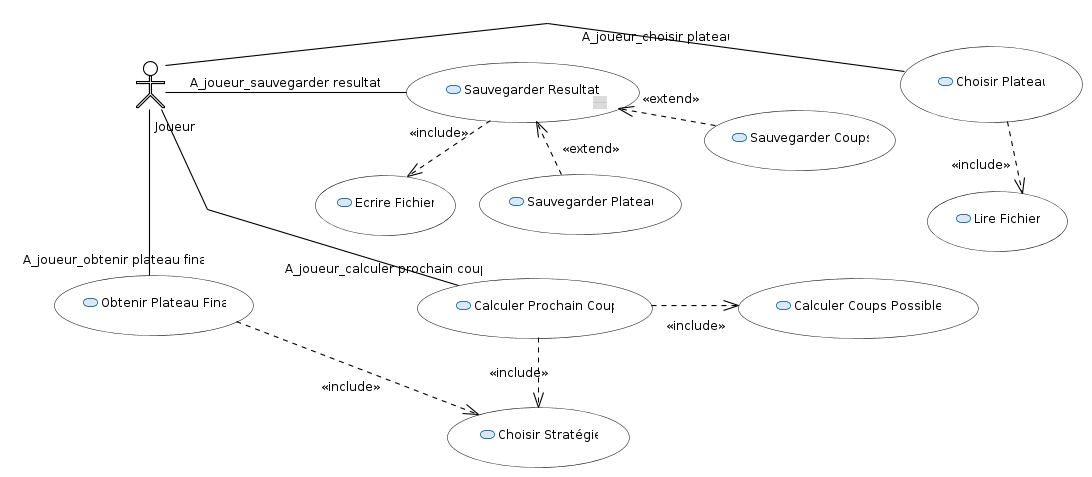
\includegraphics[scale=0.55]{images/diagramme_utilisation}
\caption{Diagramme de cas d'utilisation.}
\label{fig:cas_utilisation}
\end{figure}

\subsection{Diagramme de classes}

Une fois tous les besoins identifiés, on peut penser aux détails, c'est-à-dire,
leurs méthodes et variables, qui concernent les classes qui feront partie de
notre application. Tout d'abord, nous avons considéré de diviser nos classes
selon leurs caractéristiques et les placer dans trois groupes, étant ainsi:

\begin{itemize}
  
  \item \textbf{Entités}: les classes placées dans ce groupe répresentent les
  données et encapsulent les données utilisées. Ces classes seront naturellement
  utilisées dans tous les autres groupes de l'application. On cite notamment les
  classes \textit{Plateau} et \textit{Coup} qui contiennent respectivement les
  données nécessaires à la répresentation d'un plateau et d'un coup.
  
  \vspace{12pt}
  
  \item \textbf{Contrôle}: ce groupe contient les classes responsables pour
  contrôler le déroulement du jeu. Elles sont ainsi capables de contrôler les
  interfaces, de décider les prochains coups et contiennent les variables qui
  décrivent l'état actuel du jeu.
  
  \vspace{12pt}
  
  \item \textbf{Interfaces}: les dernières classes sont engagées à l'interface
  entre l'utilisateur final, soit à travers du terminal, soit par fênetres. On
  place également dans cette classification, la classe dédiée à la manipulation
  des fichiers.
  
\end{itemize}

\vspace{12pt}

Le résultat est finalement montré dans figure \ref{fig:diagramme_classes} de la
section \textbf{Annexes}.

\subsubsection{Les classes \og Entités \fg}

Comme abordé précédemment, les classes qui appartiennent à ce groupe possèdent
les informations importantes qui seront utilisées par toutes les autres
structures de l'application. En d'autres mots, ce sont des données fondamentales
à d'autres classes et aux algorithmes d'intelligence artificielle. La figure
\ref{fig:classes_entites} montre en détail les components de ce paquet.

\begin{figure}[h]
\centering
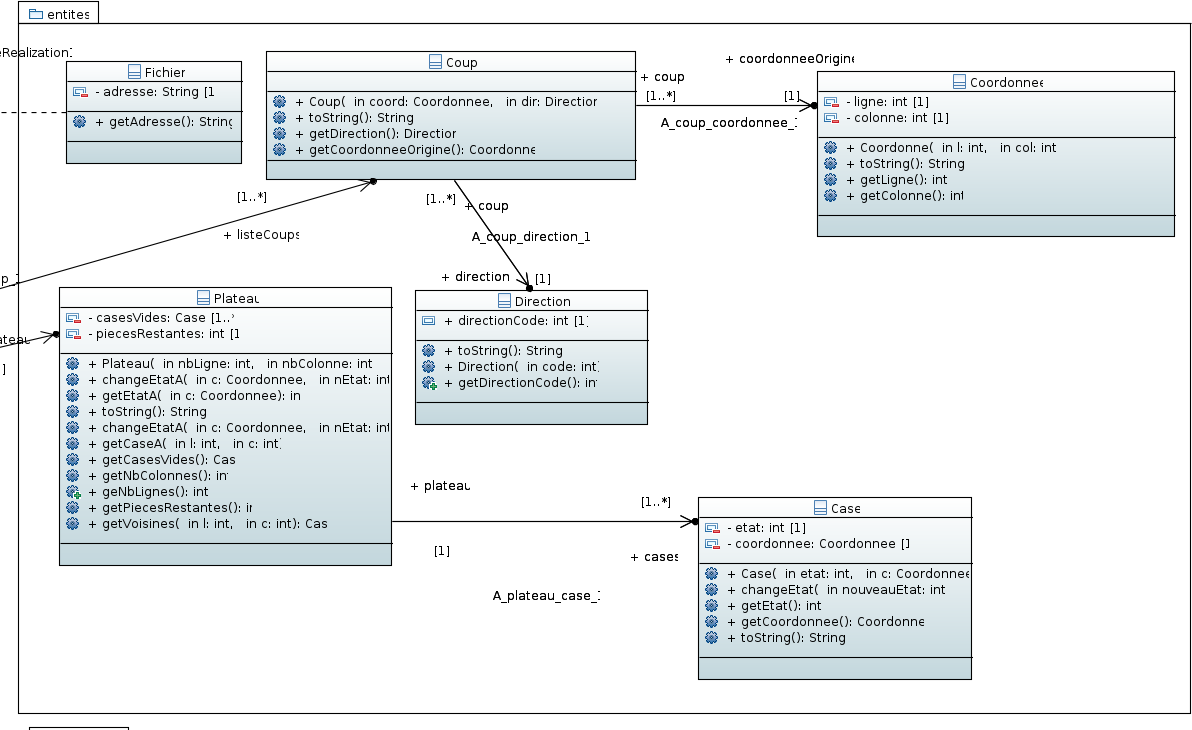
\includegraphics[scale=0.45]{images/entites}
\caption{Paquetage \og entités \fg ~du diagramme de classes.}
\label{fig:classes_entites}
\end{figure}

On peut notamment citer:

\vspace{12pt}

\begin{itemize}
  \item La classe \textbf{Plateau} contient les informations qui décrivent
  complétement un plateau de taille et nombre de pions quelconque. Elle garde
  aussi une liste avec les cases actuellement vides et le nombre de pièces
  restantes. C'est à un objet de cette classe gérer les changements d'état des
  ses cases, gardées sur une matrice d'objets de type Case.
  
  \vspace{12pt}
  
  \item Chaque objet appartenant à classe \textbf{Case} a un attribut qui
  décrit son état actuel et sa coordonnée vis-à-vis au plateau. A principe, on
  a rejetté l'idée d'avoir une telle classe, puisqu'on pourrait implémenter une
  matrice des entiers directement, mais après réflechir un peu, on a décidé de la
  maintenir, vu qu'elle rendrait plus facile le codage des algorithmes et un
  possible changement de la structure de données (par exemple, si on voulait
  remplacer une liste au lieu de la matrice).
  
  \vspace{12pt}
  
  \item La classe \textbf{Coup} répresente un mouvement et possède une direction
  et une coordonnée d'origine.
  
  \vspace{12pt}
  
  \item La classe \textbf{Direction} possède un attribut entiers qui peut avoir
  seulement quatre valeurs possibles (haut, bas, droite et gauche). Sa concéption
  a été justifiée par la facilité d'écrire de méthodes comme \textit{toString}
  et de constantes qui répresentent les directions.
  
  \vspace{12pt}
  
  \item La classe \textbf{Coordonnee} répresente les valeurs d'une ligne et d'une
  colonne par rapport à la matrice qui forme le plateau.
  
  \vspace{12pt}
  
  \item  La classe \textbf{Fichier} implémente l'interface \textit{IMilieu} du
  paquet \textit{controle} (\textit{cf.} section \ref{sec:controle}) et
  répresente les données d'un fichier. On remarque que cette construction a été
  choisie pour garantir sa généralité, c'est-à-dire, si on veut étendre notre
  programme pour lire le plateau d'un serveur par exemple, ce dernier paquet
  reste inchangeable.
  
\end{itemize}

\subsubsection {Les classes \og Contrôle \fg}
\label{sec:controle}

Toutes les opérations qui concernent la gestion des données et des mouvements
sont réalisées par les classes dans ce paquet, selon figure
\ref{fig:classes_controle}. On observe la présence de trois interfaces qui
garantissent sa généralité: une fois que l'interface graphique ou la façon de
lire le plateau changent, aucune modification sera nécessaire à ce paquet. Dans
notre cas, nous avons implémente deux façons d'affichage des résultats (une via
terminal et autre via des fênetres), mais toutes les deux utilisent la même
classe \textit{ControleurJeu}.

\begin{figure}[h]
\centering
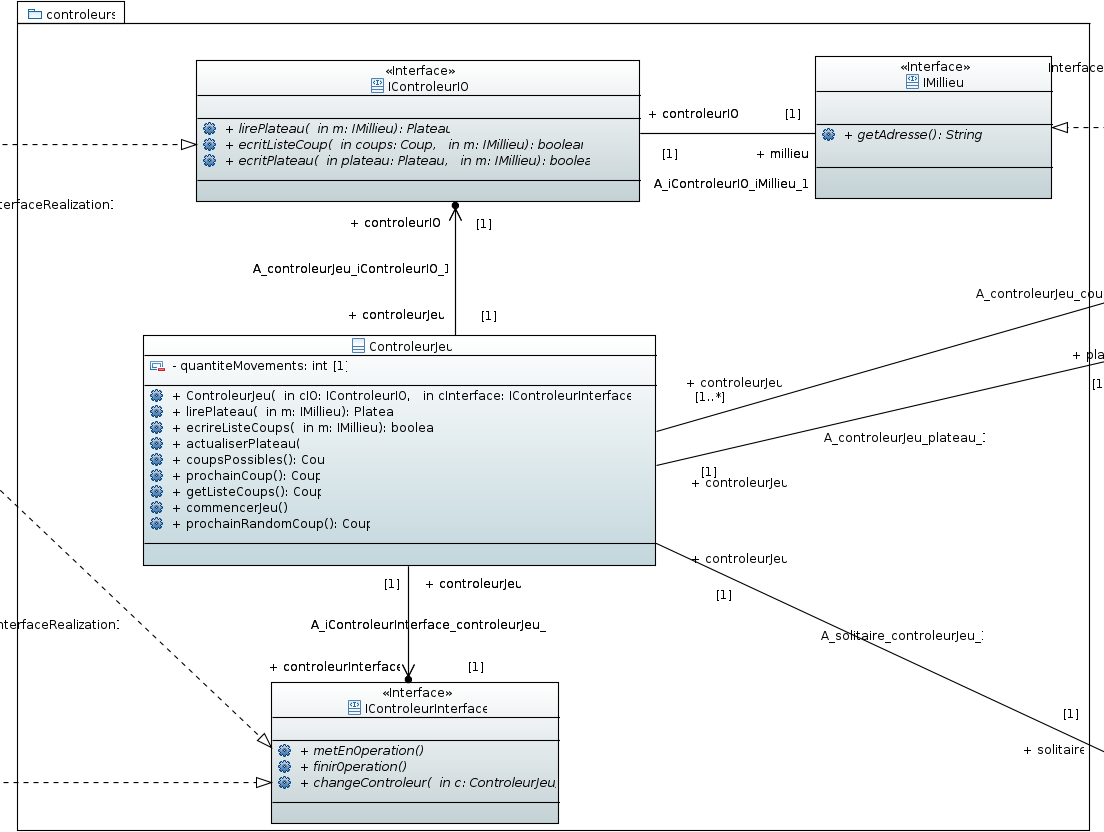
\includegraphics[scale=0.45]{images/controle}
\caption{Paquetage \og controle \fg ~du diagramme de classes.}
\label{fig:classes_controle}
\end{figure}

En ce qui concerne les fonctionnalités de chaque classe individuellement, on
observe que:

\vspace{12pt}

\begin {itemize}
  \item le classe \textbf{ControleurJeu} centralise le contrôle du jeu et,
  conséquemment, son déroulement. C'est à elle aussi d'assigner aux contrôleurs
  restants leurs respectives tâches, comme par exemple, envoyer au contrôleur
  d'entrée et sortie de messages de lecture ou écriture. Compte tenu de sa
  nature, cette classe utilise plusieurs attributs qui répresentent l'état du
  jeu, notamment la liste de coups réalisés, un plateau et la quantité de
  mouvements.
  
  \vspace{12pt}
  
  \item l'interface \textbf{IControleurInterface} défine les opérations qu'une
  classe doit fournir si elle est destinée à l'affichage des données.
  
  \vspace{12pt}
  
  \item l'interface \textbf{IControleurIO} définera ce qu'une classe
  responsable pour contrôler les opérations d'entrée et sortie devra fournir.
  Elle fait l'usage également d'une autre interface, \textbf{IMilieu}, qui
  répresente les caractéristiques d'un milieu quelconque.
\end{itemize}

\subsubsection{Les classes \og Interface \fg}

L’affichage, soit via le terminal soit via l’interface graphique, et la
communication à travers de fichiers sont réalisés par les classes de ce paquet.
La figure numéro \ref{fig:classes_inteface} montre  sa modélisation.

\begin{figure}[h]
\centering
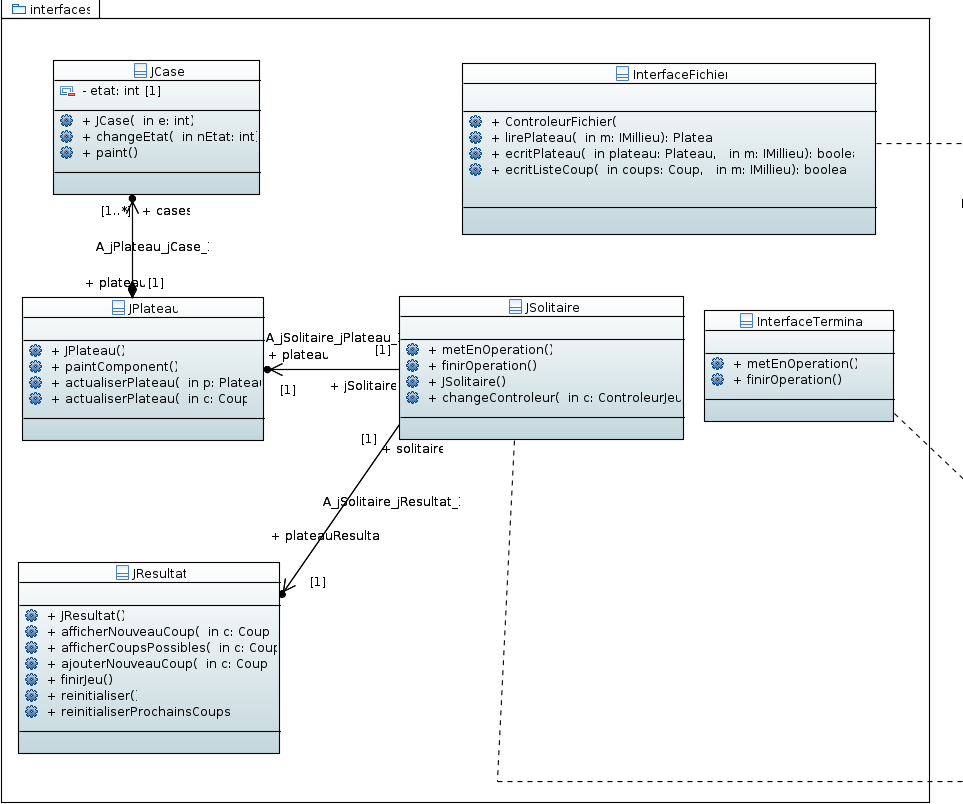
\includegraphics[scale=0.45]{images/interface}
\caption{Paquetage \og interface \fg ~du diagramme de classes.}
\label{fig:classes_inteface}
\end{figure}

On remarque que:

\begin{itemize}
  \item la classe \textbf{interfaceTerminal} est responsable d'afficher les
  plateaux et la liste des coups possibles en les écrivant en format texte sur
  le terminal. Donc, les plateaux seront affichés de la même façon qu’on les
  représente dans les fichiers .
  
  \vspace{12pt}
  
  \item a classe \textbf{interfaceFichier} s’occupe des opérations sur les
  fichiers comme l’écriture et la lecture. Elle implémente aussi l’interface 
  \textit{IControleurInterface} du paquet \textit{Contrôle}.
    
  \vspace{12pt}
  
  \item L’affichage graphique est fait par la classe \textbf{JSolitaire} et ses
  components. Elle est composée par deux parties principales: le plateau où les
  pions seront représentés et un tableau de résultats. Cette classe hérite
  \textit{JFrame} de Java qui implémente une fenêtre basique.
  
  \vspace{12pt}
  
  \item la classe \textbf{JPlateau} est responsable pour gérer l’affichage des
  pions.  Elle est composée par une matrice de \textbf{JCase} qui représente une
  seule position du plateau. Ces deux classes héritent de \textit{JPanel} fourni
  par Java et ont leurs méthodes paint redéfinies pour qu’elles puissent bien
  représenter l’état du plateau.

  \vspace{12pt}
  
  \item \textbf{JResultat} est la classe  chargé d’afficher les résultats. Elle
  fournit une liste de stratégies possibles et deux boites de texte où seront
  affichés la liste de coups déjà réalisés et la liste de coups de coups que
  sont possibles à chaque moment. Il y a aussi deux boutons, un pour réaliser un
  seul coup et l’autre pour finir le jeu selon la stratégie choisie.
  
\end{itemize}

\section{Le codage}

\subsection{L'implémentation du paquet \og Entités \fg}

Les classes de ce paquet en général ont d'implémentation simple puisque leurs
méthodes ne font que retourner l'état actuel de leurs attributs. Par conséquent,
les méthodes des objets des classes comme \textbf{Coordonnee},
\textbf{Direction}, \textbf{Fichier} et \textbf{Case} ne fournissent que les
\textit{getters} et les méthodes d'écriture \textit{toString}. Par contre, les
classes \textbf{Plateau} et \textbf{Coup} possèdent des fonctionnalités plus
importantes vis-à-vis au déroulement du programme. Par exemple, on trouve dans
ces respectives classes les fonctionnalités suivantes:

\vspace{12pt}

\begin{itemize}
  
  \item Un objet du type \textbf{Plateau} est capable de fournir des méthodes
  qui calculent toutes les cases actuellement vides, changent l'état d'une
  position quelconque et également retournent tous les voisins d'une coordonnée.
  Ces méthodes sont très utilisées par le contrôleur lors du calcul de chaque
  coup du jeu.
  
  \vspace{12pt}
  
  \item Les méthodes appartenant à la classe \textbf{Coup} s'occupent plutôt de
  rétourner les coordonnées des cases d'origine, cible et l'éliminée et aussi la
  diréction du saute.
\end{itemize} 

\subsection{L'implémentation du paquet \og Contrôle \fg}

Ce paquet ne contient que trois components: deux interfaces et une classe, la
plus importante de tout le programme, puisqu'elle doit gérer le fonctionnement
de tous les éléments de l'application. Les interfaces ne font que fournir des
méthodes qu'une classe doit implémenter pour être utilisée. Ainsi, toute
classe qui a comme but afficher le plateau et les résultats doit avoir des
méthodes qui permettent une communication entre elle-même et le contrôleur.

\vspace{12pt}

En ce qui concerne les outils fournis par \textbf{ControleurJeu}, on remarque:

\vspace{12pt}

\begin{itemize}
  
  \item Le calcul d'un prochain coup selon une stratégie les entre neuf
  implémentées (voir section \ref{sec:strategie}). 

  \vspace{12pt}
  
  \item Gérer les contrôleurs d'affichage et d'éntrée/sortie.
  
  \vspace{12pt}
  
  \item Garder et maintenir l'état du jeu toujours consistent.
   
\end{itemize}

\subsubsection{Stratégies de résolution}
\label{sec:strategie}

On divise les neuf stratégies développées en trois groupes, étant eux: 
\vspace{12pt}

\begin{itemize}

  \item Stratégies s'appuyant sur des critères locaux: dans ce groupe, on trouve
  des stratégies qui utilisent de caractéristiques par rapport à l'état actuel
  du plateau. En d'autre mots, elles n'essayent pas de trouver un parcours
  optimal entre plusieurs. Les critères jugés les plus importants ont été alors:

  \vspace{12pt}
  \begin {itemize}
  
	  \item Nombre de voisins de la case finale: on choisit le couple dont
	  réalisation donne une case avec le nombre le plus grand de
	  voisins autour de soi. De cette façon, on préfère toujours les coups qui
	  auront plus de possibilités d'avoir d'autres coups dans l'avenir.
	  L'algorithme qui considère le nombre le plus petit a été fait également, mais
	  seulement pour tester les différentes solutions.
  	  
  	  \vspace{12pt}
  	  
  	  \item Distance par rapport au dernier coup réalisé: l'idée est de
  	  prendre un coup le plus distant possible du coup qui vient d'être fait. De cette
  	  façon, on espère avoir un équilibre de la quantité des pièces partout le
  	  plateau. On a également écrit l'algorithme qui fait l'opposé, c'est-à-dire,
  	  prefère les coups les plus proches et d'avoir les coups concentrés dans une
  	  partie du plateau.
  	  
  	  \vspace{12pt}
  	  
  	  \item Distance du coup par rapport au centre: l'idée de cet algorithme est
  	  de prendre les coups qui, si réalisés, vont approcher les pièces du centre
  	  du plateau. 
  \end {itemize}
  
  \vspace{12pt}
  
  \item Stratégies s'appuyant sur des critères globaux: les algorithmes
  appartenant à ce groupe vérifient plusieurs solutions possibles et les
  comparent.
  
  \vspace{12pt}
  \begin {itemize}
    \item Chercher la solution optimale (\textit{backtracking}): la base de cet
    algorithme est de explorer récursivement tout les coups possibles du jeu,
    afin de trouver la solution contenant le maximum de coups. Évidémment, cet
    algorithme devient impraticable pour des plateau grands à cause de sa
    haute complexité.
    
	\vspace{12pt}
	
    \item La technique \textit{Branch and Bound}: l'algorithme consiste à
    chercher la liste de coups la plus grande possible en se baseant sur
    les tailles des sous-arbres que chaque coup possible peut avoir à chaque
    niveau d'itération. Par exemple, si à un instant donné, on a trois coups
    possibles, l'algorithme, pour chaque coup, va choisir et calculer la taille
    d'une des leurs sous-arbres et, une fois fini, il va les comparer. La
    sous-arbre choisie est alors la plus longue. On remarque encore qu'on a
    décidé de construire aléatoirement chaqu'une des sous-arbres.  
    
  \end{itemize}  
  
  \vspace{12pt}
  
  \item Autres stratégies: on a encore implementé certains algorithmes qui
  utilisent les méthodes décrites précédemment de façon mélangée. On cite:
  
  \vspace{12pt}
  
  \begin {itemize}
    
    \item Mélanger l'algorithme de \textit{Branch And Bound} avec la recherche
    de la solution optimale: on commence la recherche par la méthode de
    \textit{Branch And Bound} et, lorsqu'on arrive à une déterminée quantité
    de pièces restantes, on finit avec l'algorithme qui compare toutes les
    solutions possibles.
    
	\vspace{12pt}
	
    \item Réalisation de \textit{Branch and Bound} plusieurs fois: on éxécute
    cet algorithme plusieurs fois et prend la liste de coups la plus grande
    entre les résultats.
    
    \vspace{12pt}
    
    \item Réalisation de \textit{Branch and Bound} avec des niveaux de
    profondeur: différemment de l'algorithme précédent, on parcourt chaque
    sous-arbre, qui répresente essentiellement un nouveau plateau, et après   
    être arrivé à la profondeur choisie, on calcule le coups suivants avec l'un
    des nos algorithmes déjà présentés. Le choix de la profondeur dépend
    évidemment de la taille du plateau original puisque le temps de calcul est
    directement relié à la quantité de coups possibles à chaque niveau, ce qui
    augmente dans les cas des grands plateaux.
        
  \end{itemize}

\end{itemize}

\vspace{12pt}
 
 Après quelques essais, on a conclu que la dernière stratégie présente les
 meilleurs résultats.
 
\subsection{L'implémentation du paquet \og Interface \fg}

Les dernières classes à être codées sont les classes qui vont
effetivement afficher les résultats et écrire/lire des fichiers.

\subsubsection {L'interface graphique} 

L'interface graphique a été conçue entièrement à partir des bibliotèques
\textit{swing} et \textit{awt} fournies par \textit{Java}, plus précisement des
classes \textbf{JFrame} et \textbf{JPanel}, qui servent de \textit{super classe}
à certaines de nos classes, comme \textbf{JSolitaire} et
\textbf{JPlateau}/\textbf{JResultat} respectivement. Le résultat se trouve
affiché par la figure \ref{fig:screen}.

\vspace{12pt}

Outre son héritage, la classe JSolitarie implémente également l'interface
\textbf{ActionListener}, qui lui permet de savoir et traiter l'événement généré
par un possible click sur un des boutons. Cette classe est composée par un
plateau - un objet \textbf{JPlateau} - et un panneau de résultats - du type
\textbf{JResultat}. Ces deux components sont placés sur l'espace disponible de
fênetre selon les directives d'un \textit{layout manager}. Dans ce cas, on a
utilisé un simple \textbf{BorderLayout} qui n'impose pas de grandes difficultés
de configuration mais, par compensation, n'offre pas un contrôle très précis des
ses components.

\vspace{12pt}

La classe \textbf{JPlateau} contient une matrice de components \textbf{JCase},
qui héritent également de \textbf{JPanel}. Cette matrice est évidemment
une réflexion de la matrice contenue dans un objet du type
\textbf{ControleurJeu}. En ce qui concerne le \textit{layout manager},
appelé \textbf{GridLayout}, on remarque qu'il joue un rôle fondamental puisque
c'est lui le responsable pour diviser et mettre l'écran en forme matricielle.
En conséquence, nous sommes épargnés de certains calculs chaque fois qu'on doit
modifier les dimensions du plateau. Le dernière caractéristique importante
consiste à modifier la méthode \textit{paintComponent} pour qu'elle puisse
appeler l'opération \textit{paint} de chaque objet \textbf{JCase}. Cette
dernière ne fait que dessiner un cercle peint en fonction de l'état.

\vspace{12pt}

Le dernier remarque consiste à noter que, à principe, on n'aurait pas besoin de
construire une nouvelle classe pour répresenter une case. On pourrait n'avoir
qu'une seule matrice d'entiers pour garder l'état. Cependant, cette
configuration présente un problème, puisqu'on ne serait pas capable d'appeler la
méthode \textit{paint} lors d'une modification. En conséquence, on serait obligé
à calculer \og à la main \fg toutes les coordonnées à chaque fois. 
 
\begin{figure}[h]
\centering
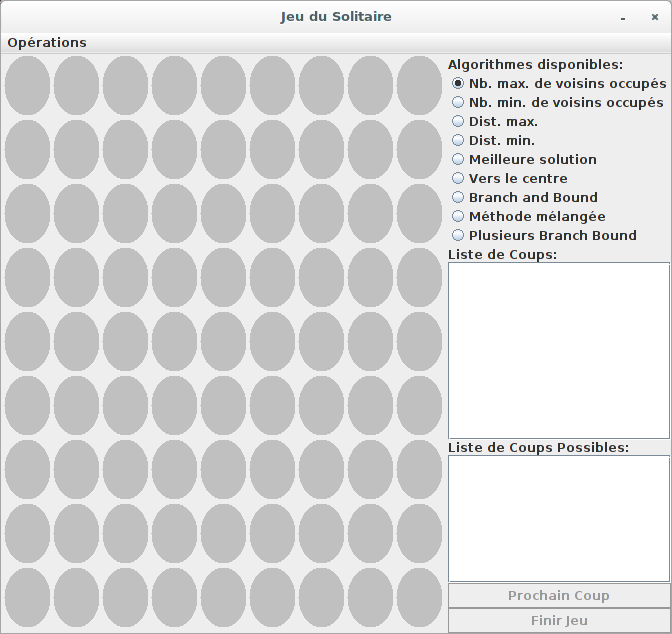
\includegraphics[scale=0.35]{images/screen}
\caption{Interface graphique.}
\label{fig:screen}
\end{figure}

\subsubsection {L'interface d'entrée et sortie}

Afin de lire et écrire sur les fichiers on a utilisé les classes
\textbf{BufferedReader} et \textbf{FileWriter} respectivement. Toutes les deux
peuvent lancer une exception si le fichier qu'on essaie de lire ou
écrite n'existe pas. Dans ce cas, on a choisi de les traiter à niveau de la
classe \textbf{JSolitaire}, qui peut, à son tour, afficher une boîte
d'information en communiquant l'erreur.

\newpage
\section{Annexes}

\begin{figure}[h]
\centering
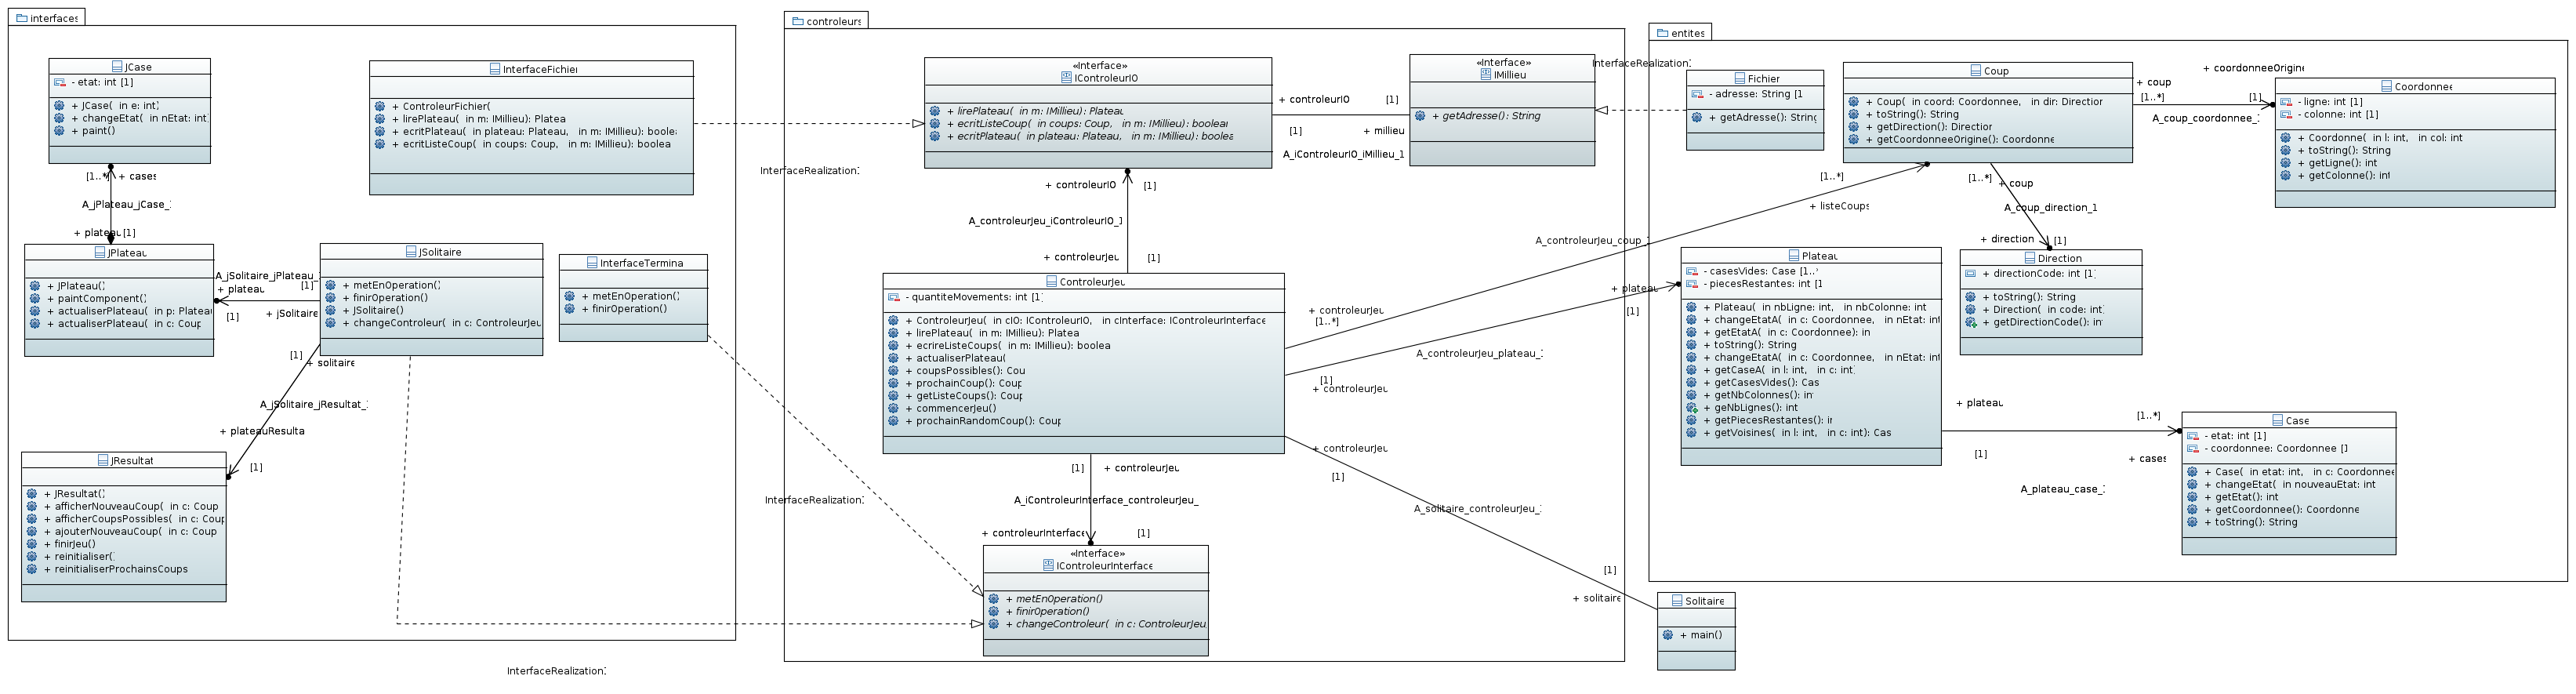
\includegraphics[angle=-90, scale=0.19]{images/diagramme_classes}
\caption{Diagramme de classes.}
\label{fig:diagramme_classes}
\end{figure}

\end{document}
